% !TEX TS-program = xelatex
% !TEX encoding = UTF-8 Unicode
% !Mode:: "TeX:UTF-8"

\documentclass{resume}
\usepackage{graphicx}
\usepackage{tabu}
\usepackage{tabularx}
\usepackage{multirow}
\usepackage{progressbar}
\usepackage{zh_CN-Adobefonts_external} % Simplified Chinese Support using external fonts (./fonts/zh_CN-Adobe/)
\usepackage{tikz}
% \usepackage{NotoSansSC_external}
% \usepackage{NotoSerifCJKsc_external}
% \usepackage{zh_CN-Adobefonts_internal} % Simplified Chinese Support using system fonts
\usepackage{linespacing_fix} % disable extra space before next section
\usepackage{cite}

\newcommand{\hlink}[1]{\href{#1}{#1}}

\begin{document}
\pagenumbering{gobble} % suppress displaying page number

\medskip\noindent
\begin{minipage}{0.7\textwidth}
  \Large{
    \begin{tabu}  { l }
      \scshape{徐 \quad  颖} \\
      \email{xuying1706@buaa.edu.cn} \\
      \phone{(+86) 131-2661-1215} \\
    \end{tabu}
  }
\end{minipage}
\begin{minipage}{0.3\textwidth}
  \raggedleft
  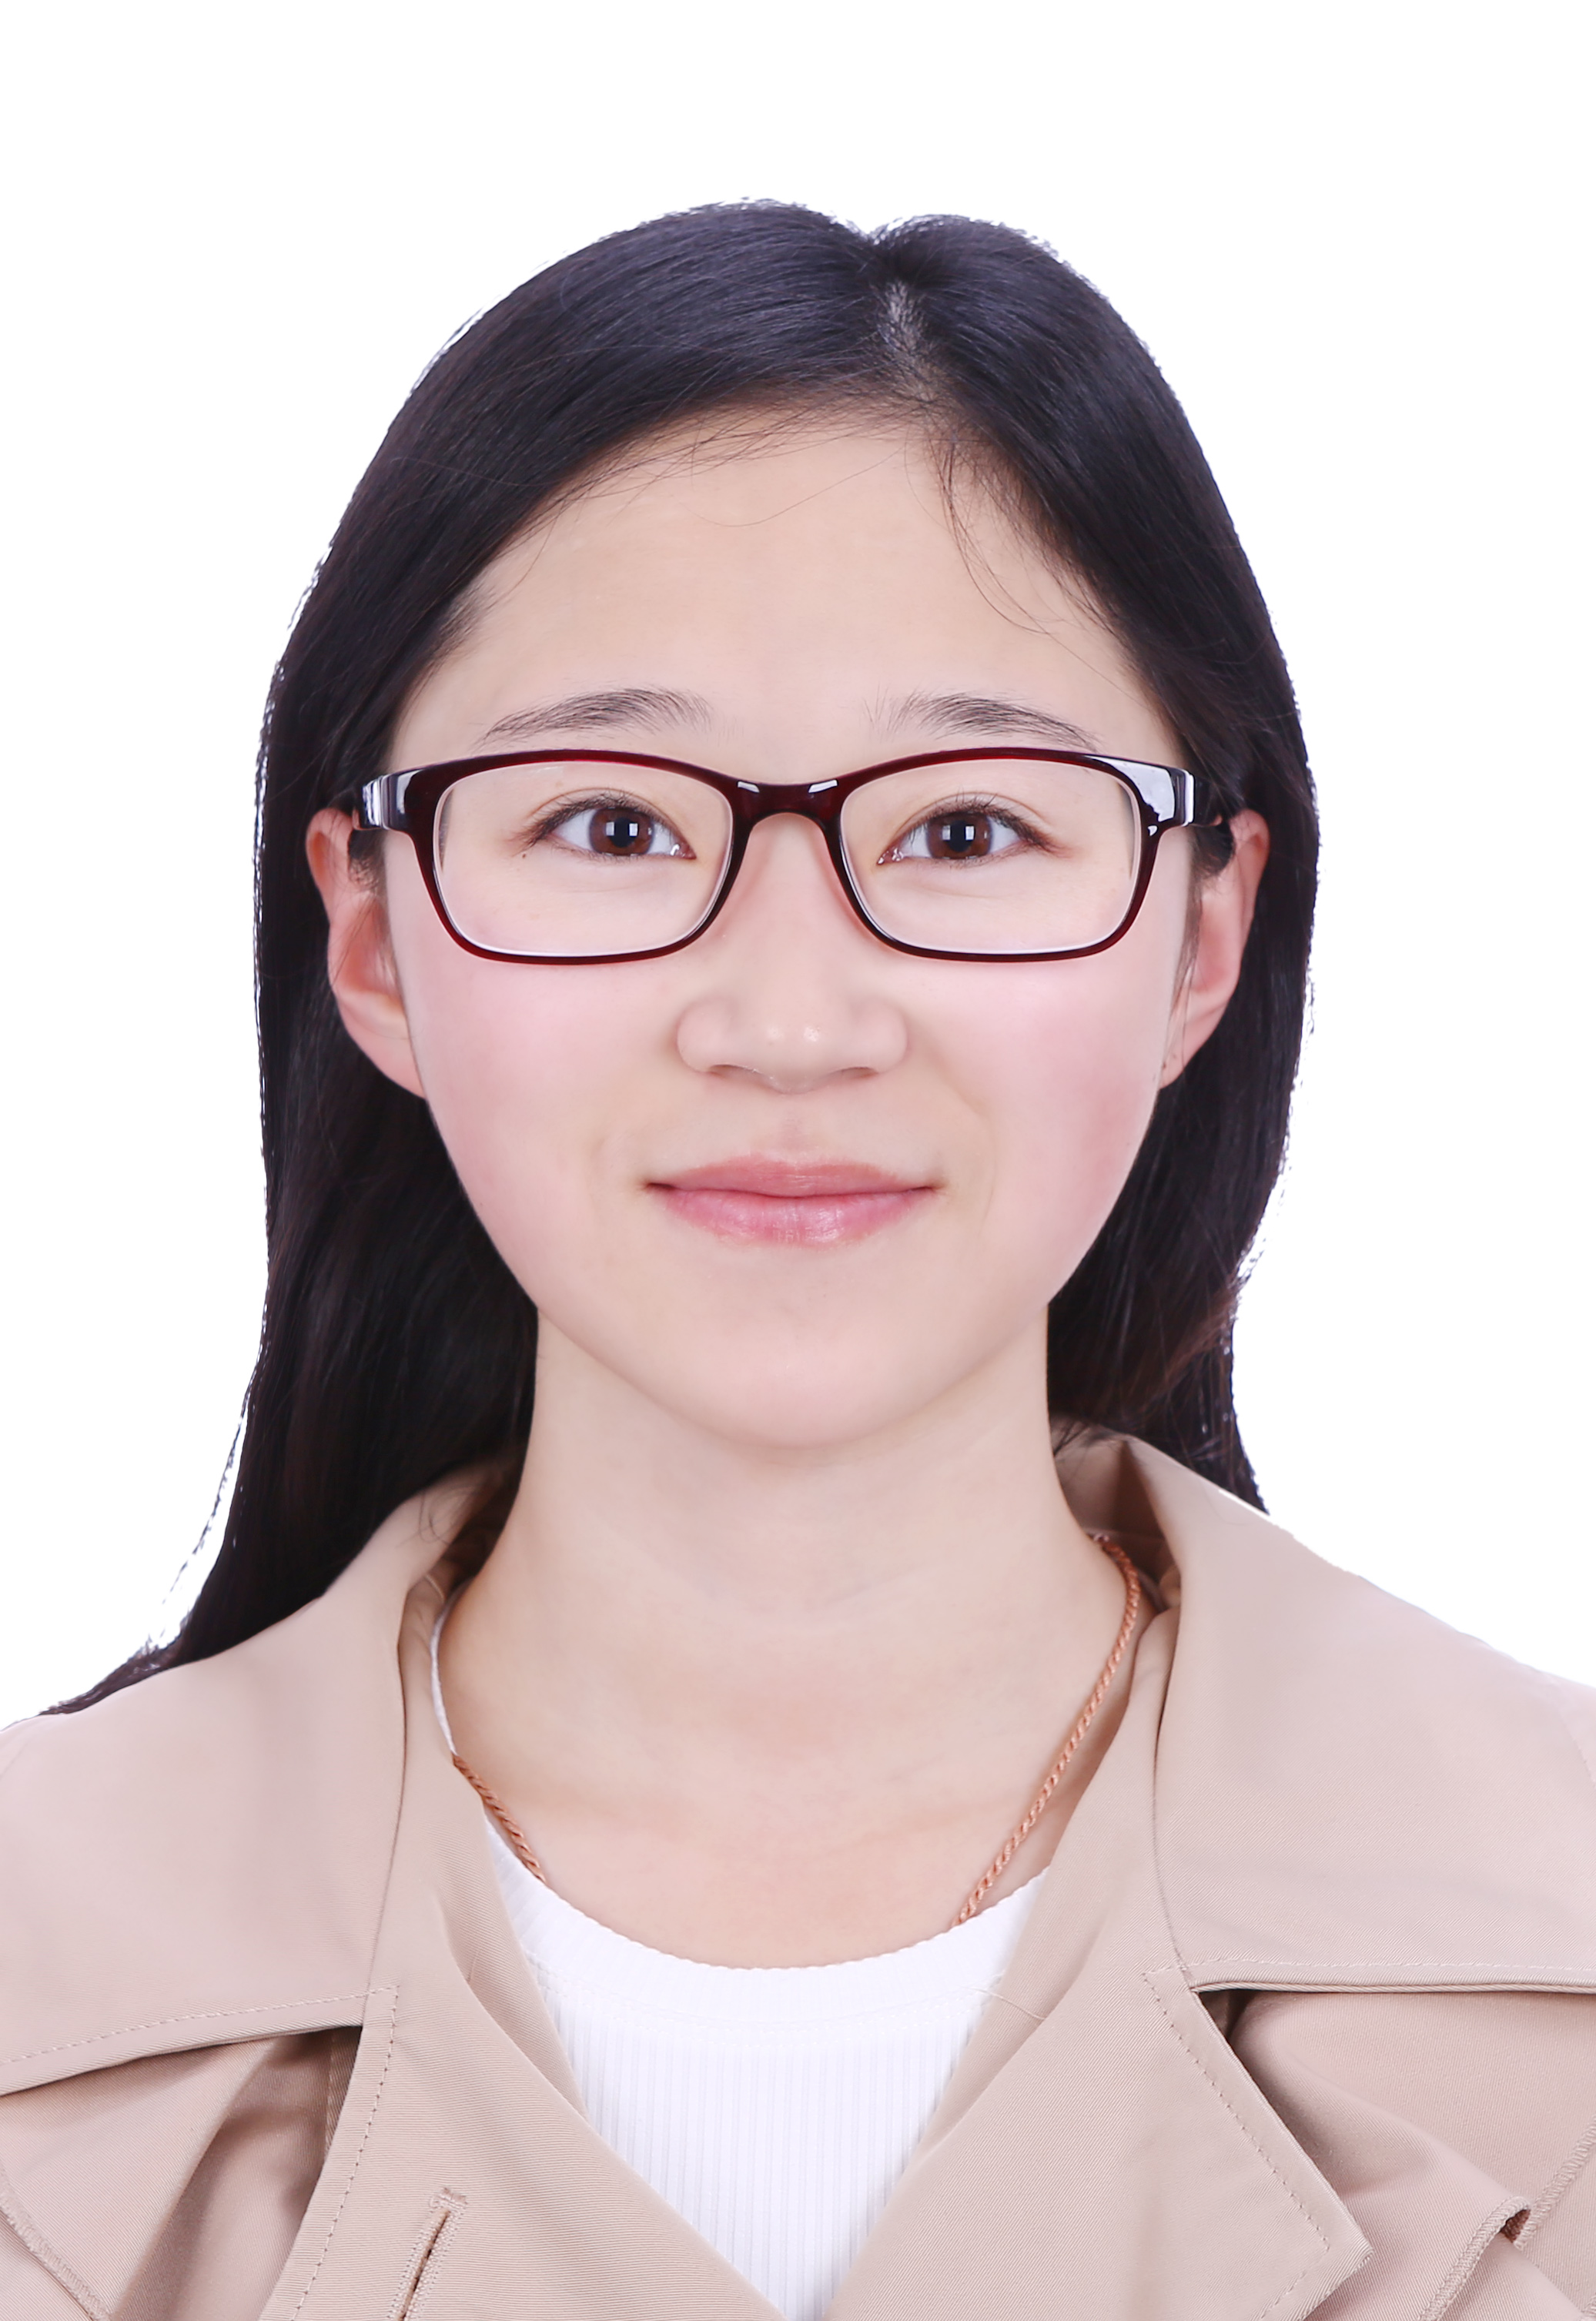
\includegraphics[height=30mm]{xy}
\end{minipage}

\section{  教育背景}
\datedsubsection{\textbf{北京航空航天大学}, 北京}{2017.08 -- 至今}
\textit{在读硕士研究生}\quad {计算机学院,智能识别与图像处理实验室}
%\begin{onehalfspacing}
\begin{itemize}[topsep = 0 pt, partopsep = 0pt]
  \item  主修课程:模式识别、密码学
\end{itemize}
%\end{onehalfspacing}
\datedsubsection{\textbf{南开大学}, 天津}{2013.09 -- 2017.07}
\textit{学士}\quad  {计算机与控制工程学院}
%\begin{onehalfspacing}
\begin{itemize}[topsep = 0 pt, partopsep = 0pt]
  \item 主修课程:C++、数据库系统原理、信息检索
\end{itemize}
%\end{onehalfspacing}

\section{  项目经历}

\datedsubsection{\textbf{对抗攻击}}{2018.10 -- 至今}
\role{研究生课题}{}
%\begin{onehalfspacing}
\begin{itemize}[topsep = 0 pt, partopsep = 0pt]
  \item 使用DAG算法对FCN和Faster-RCNN进行攻击
  \item 使用GAN对Two-Stream动作识别模型进行攻击
\end{itemize}
%\end{onehalfspacing}


\datedsubsection{\textbf{目标检测}}{2018.02 -- 2018.09}
\role{研究生课题}{}
%\begin{onehalfspacing}
\begin{itemize}[topsep = 0 pt, partopsep = 0pt]
  \item 使用Faster-RCNN和Mask RCNN进行目标检测
\end{itemize}
%\end{onehalfspacing}

\datedsubsection{\textbf{基于时空分解的民航旅客流量分析与预测}}{2016.06 -- 2017.06}
\role{本科毕设}{}
\begin{itemize}[topsep = 0 pt, partopsep = 0pt]
  \item 对民航客流量大数据进行清洗和统计
  \item 深入分析民航旅客在时间和空间上的出行规律
  \item 建立民航领域的时空残差网络模型,对航线的日客流量进行预测
\end{itemize}

\section{学生工作}
  \datedline{\textit{CCF北航学生分会主席}}{2018.12 -- \  \quad 至今}
  \datedline{\textit{CCF北航学生分会副主席}}{2017.11 -- 2018.12}
  \datedline{\textit{南开大学360俱乐部组织部组长}}{2015.03 -- 2017.06}
  \datedline{\textit{南开大学豌豆藤志愿服务组织小组组长}}{2013.10 -- 2017.06}

\section{技能}
  \datedline{\textit{语言: CET-6 547}}
  \datedline{\textit{编程语言: 掌握C++、MATLAB、Python,了解SQL}}
  \datedline{\textit{框架: PyTorch、Caffe}}
  \datedline{\textit{工具: Linux、Git、MySQL、SQL Server}}

\section{获奖情况}
  \datedline{\textit{北京航空航天大学研究生学业奖学金}}{2018.08}
  \datedline{\textit{北京航空航天大学研究生新生奖学金}}{2017.08}

\end{document}
